%%%%%%%%%%%%%%%%%%%%%%%%%%%%%%%%%%%%%%%%%%%%%%%%%%%%%%%%%%
%% SLIDE 3: CUSTOMER JOURNEY
%%%%%%%%%%%%%%%%%%%%%%%%%%%%%%%%%%%%%%%%%%%%%%%%%%%%%%%%%%

\begin{frame}
    \begin{tikzpicture}[remember picture,overlay]
    \fill[PrimaryBlueLighter, opacity=0.08] ([xshift=-3cm,yshift=2cm]current page.south east) circle (4cm);
    \fill[PrimaryGoldLight, opacity=0.06] ([xshift=4cm,yshift=-2cm]current page.north west) circle (3.5cm);
    \node[anchor=north west, text=FundoQuestion, font=\bfseries\tamanhoQuestion\selectfont]
    at ([xshift=0.8cm,yshift=-0.8cm]current page.north west) {What valuable information disappears during a purchase?};
    \node[anchor=north west, text width=.80\paperwidth, align=left, text=FundoKeyMessage, font=\tamanhoKeyMessage\selectfont]
    at ([xshift=0.8cm,yshift=-1.6cm]current page.north west) {
    Retailers see what customers buy, but much of what they considered before buying is lost.
    };
    \end{tikzpicture}

    \vspace{0.0cm}

    \begin{columns}[T, onlytextwidth]
        % Coluna da esquerda - Título com impacto visual
        \begin{column}{0.25\textwidth}
            \vspace{0.5cm}
            {\Huge\bfseries\textcolor{PrimaryGold}{Precious}}\\[0.2cm]
            {\huge\bfseries\textcolor{PrimaryBlue!80!PrimaryGold}{Data}}\\[0.3cm]
            {\LARGE\bfseries\textcolor{PrimaryBlue}{That}}\\[0.2cm]
            {\huge\bfseries\textcolor{PrimaryBlue!70!black}{Gets}}\\[0.3cm]
            {\Huge\bfseries\textcolor{PrimaryRed}{Lost}}
        \end{column}
        
        % Coluna da direita - Imagem
        \begin{column}{0.80\textwidth}
            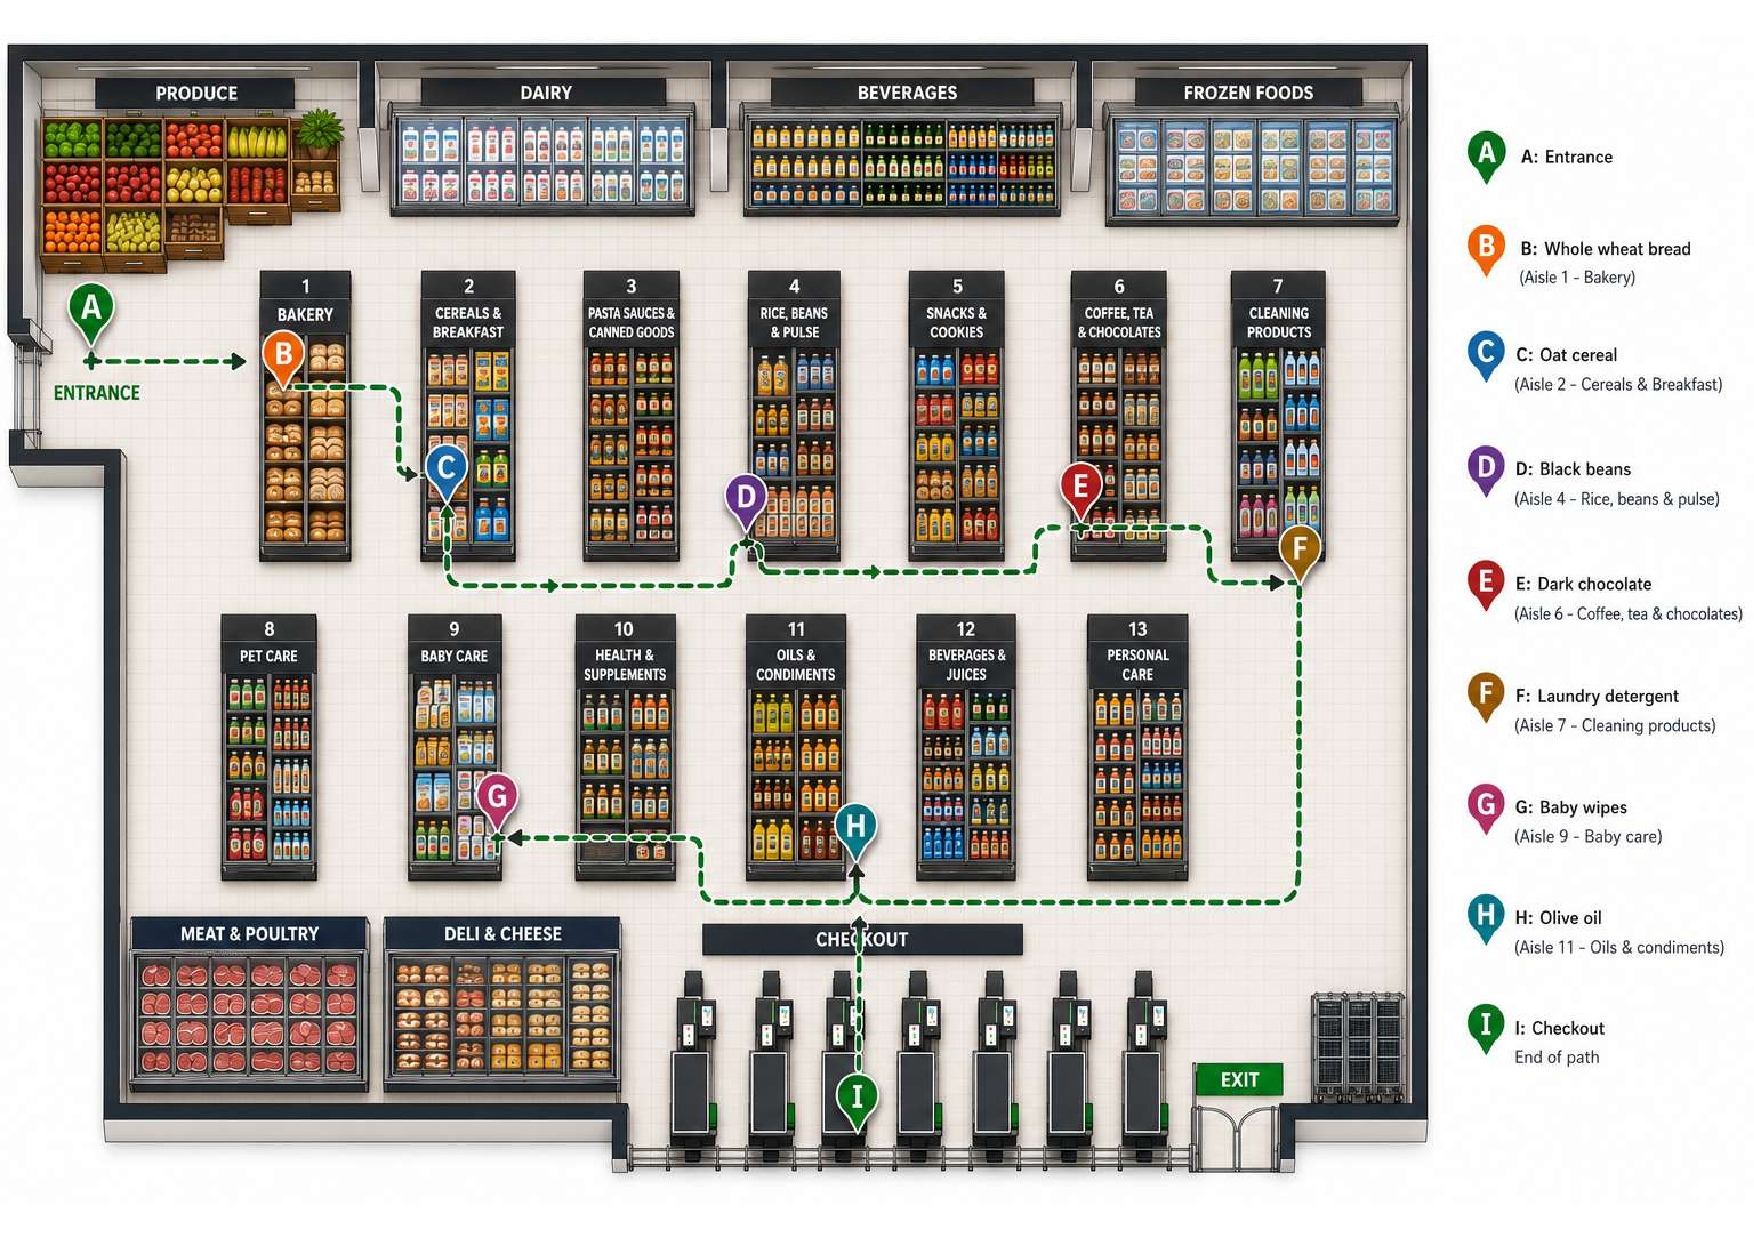
\includegraphics[width=\textwidth, keepaspectratio]{Images/Clients_Journey.pdf}
        \end{column}
    \end{columns}

\end{frame}